\documentclass[12pt]{article}


\usepackage{amssymb}
\usepackage{amsmath}
\usepackage{fullpage}
\usepackage{epsfig}
\usepackage{epstopdf}
\everymath{\displaystyle}
\usepackage{enumerate}

\newif\ifans

\anstrue

\begin{document}

\begin{center}
\underline{\LARGE{Chapter 3.2: Definition of Trigonometric Functions}}
\end{center}

\subsection*{Expected Skills:}

\begin{itemize}

\item Be able to define $\sin{\theta}$, $\cos{\theta}$, $\tan{\theta}$, $\sec{\theta}$, $\csc{\theta}$, and $\cot{\theta}$.

\item Be able to determine the domain and range of the 6 trigonometric functions.

\item Be able to evaluate the 6 trig functions (if defined) at the quadrantal angles or angles related to $30^\circ$, $45^\circ$, and $60^\circ$.

\item Be able to use the trigonometric identity $\sin^2\theta+\cos^2\theta=1$ and other given information to evaluate all 6 trigonometric functions.

\end{itemize}

\subsection*{Practice Problems: }

\begin{enumerate}

\item Label all of the indicated points on the unit circle, shown below.  Also, convert all of the angles from radian measurement to degree measurement.

\begin{center}
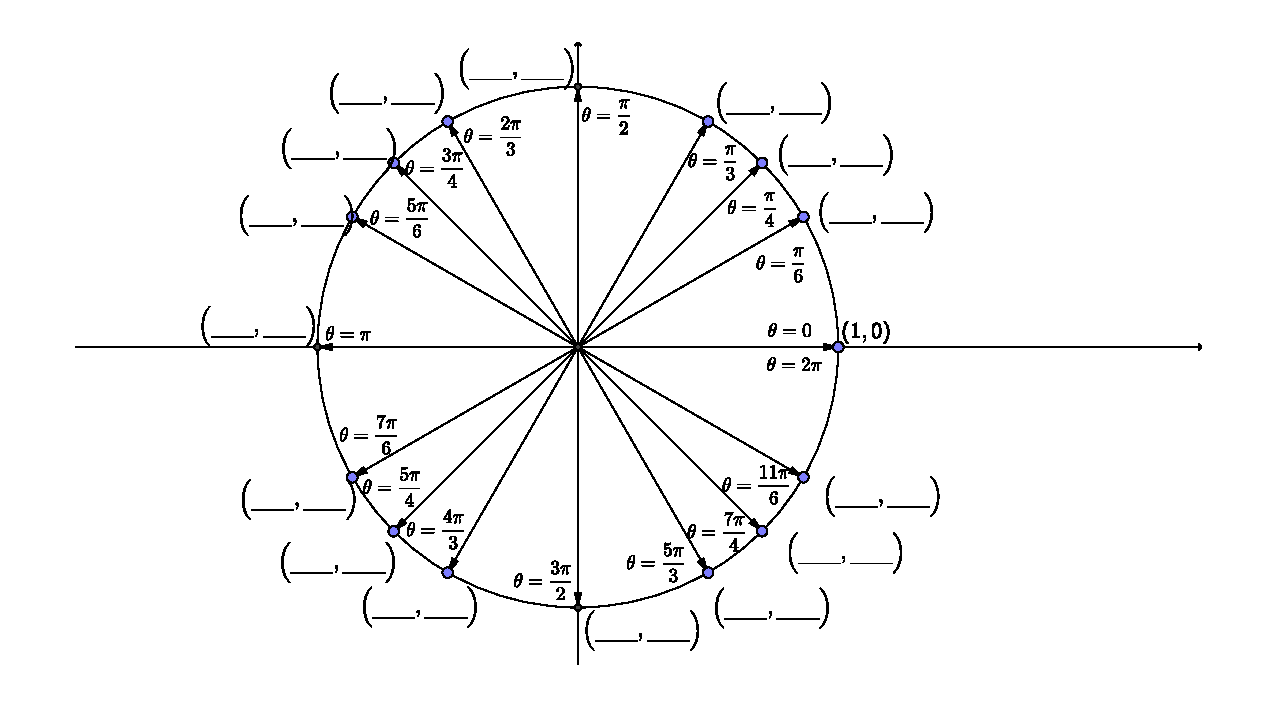
\includegraphics[scale=0.8]{unitcircle4.pdf}
\end{center}

\ifans{\fbox{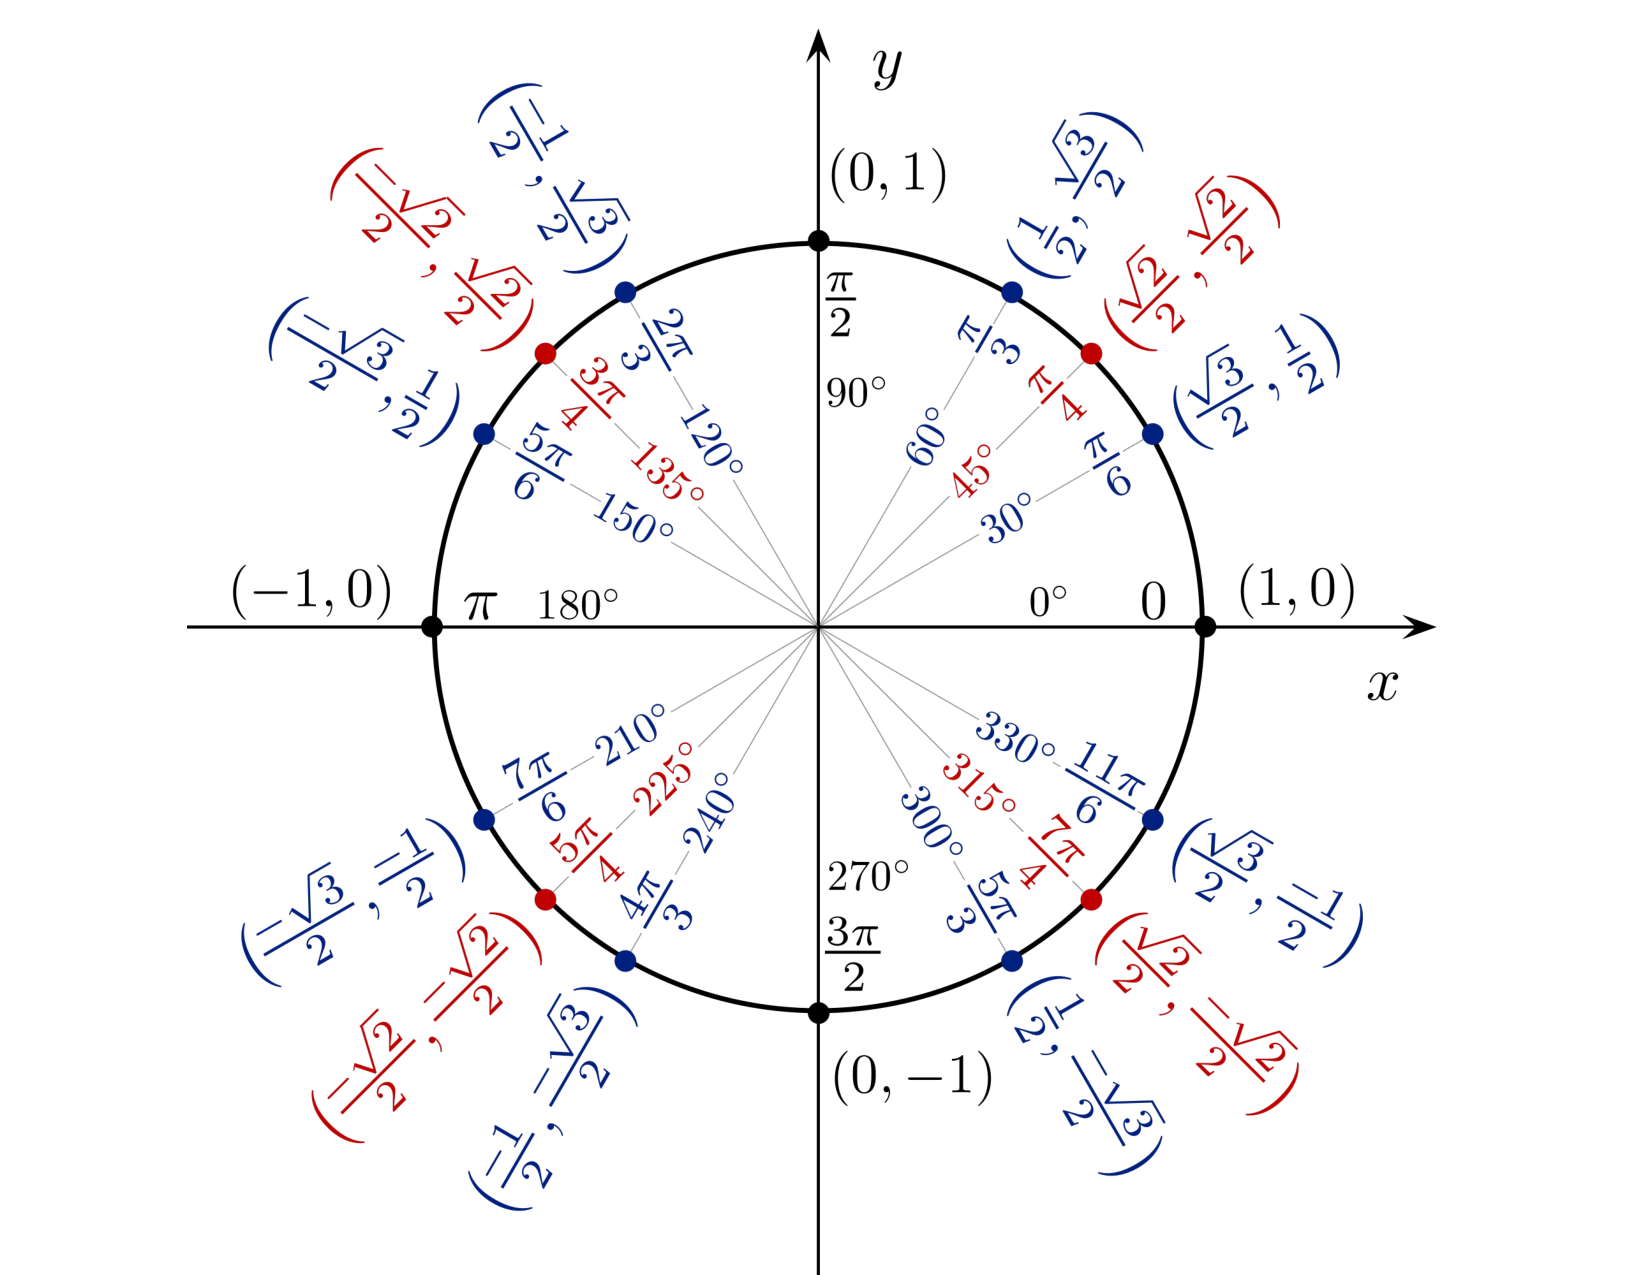
\includegraphics[scale=0.5]{unit_circle.pdf}}} \fi

\item Use your results from question (1) to evaluate each of the following without using a calculator.

\begin{enumerate}

\item $\sin{225^\circ}$

\ifans\fbox{$-\frac{1}{\sqrt{2}}$}\fi

\item $\cos{240^\circ}$

\ifans\fbox{$-\frac{1}{2}$}\fi

\item $\tan{30^\circ}$

\ifans\fbox{$\frac{1}{\sqrt{3}}$}\fi

\item $\sec{\frac{11\pi}{6}}$

\ifans\fbox{$\frac{2}{\sqrt{3}}$}\fi

\item $\cot{\frac{\pi}{2}}$

\ifans\fbox{$0$}\fi

\item $\sin{\left(-\frac{4\pi}{3}\right)}$

\ifans\fbox{$\frac{\sqrt{3}}{2}$}\fi

\item $\csc{(-690^\circ)}$

\ifans\fbox{$2$}\fi

\item $\cos{\frac{23\pi}{3}}$

\ifans\fbox{$\frac{1}{2}$}\fi

\end{enumerate}

\item Use your results from question (1) to find all solutions in the interval $[0,2\pi)$ to the following equations.

\begin{enumerate}

\item $\sin{\theta}=1$

\ifans\fbox{$\theta=\frac{\pi}{2}$}\fi

\item $\cos{\theta}=\frac{1}{2}$

\ifans\fbox{$\theta=\frac{\pi}{3}$ or $\theta=\frac{5\pi}{3}$}\fi

\item $\sec{\theta}=2$

\ifans\fbox{$\theta=\frac{\pi}{3}$ or $\theta=\frac{5\pi}{3}$}\fi

\item $\csc{\theta}=\sqrt{2}$

\ifans\fbox{$\theta=\frac{\pi}{4}$ or $\theta=\frac{3\pi}{4}$}\fi

\item $\tan{\theta}=0$

\ifans\fbox{$\theta=0$ or $\theta=\pi$}\fi

\end{enumerate}

\item Repeat question (3) providing all solutions in the interval $[2\pi,4\pi)$.

\begin{enumerate}

\item $\sin{\theta}=1$

\ifans\fbox{$\theta=\frac{5\pi}{2}$}\fi

\item $\cos{\theta}=\frac{1}{2}$

\ifans\fbox{$\theta=\frac{7\pi}{3}$ or $\theta=\frac{11\pi}{3}$}\fi

\item $\sec{\theta}=2$

\ifans\fbox{$\theta=\frac{7\pi}{3}$ or $\theta=\frac{11\pi}{3}$}\fi

\item $\csc{\theta}=\sqrt{2}$

\ifans\fbox{$\theta=\frac{9\pi}{4}$ or $\theta=\frac{11\pi}{4}$}\fi

\item $\tan{\theta}=0$

\ifans\fbox{$\theta=2\pi$ or $\theta=3\pi$}\fi

\end{enumerate}

\item Suppose $\sin{\theta}=\frac{5}{13}$ and $\frac{\pi}{2} \leq \theta \leq \pi$.  Compute the values of $\cos{\theta}$, $\tan{\theta}$, $\sec{\theta}$, $\csc{\theta}$, and $\cot{\theta}$.

\ifans\fbox{$\cos{\theta}=-\frac{12}{13}$, $\tan{\theta}=-\frac{5}{12}$, $\sec{\theta}=-\frac{13}{12}$, $\csc{\theta}=\frac{13}{5}$, and $\cot{\theta}=-\frac{12}{5}$} \fi

\item Suppose $\cos{\theta}=\frac{5}{13}$ and $\tan{\theta}<0$.  Compute the values of $\sin{\theta}$, $\tan{\theta}$, $\sec{\theta}$, $\csc{\theta}$, and $\cot{\theta}$.

\ifans\fbox{$\sin{\theta}=-\frac{12}{13}$, $\tan{\theta}=-\frac{12}{5}$, $\sec{\theta}=\frac{13}{5}$, $\csc{\theta}=-\frac{13}{12}$, and $\cot{\theta}=-\frac{5}{12}$} \fi

\item Recall that for any angle $\theta$ it follows that $\cos^2\theta+\sin^2\theta=1$.  

\begin{enumerate}

\item Suppose $\theta\neq\pi k$ (where $k$ is an integer).  Divide the original identity by $\cos^2\theta$ to derive a trigonometric identity involving tangent and secant.

\ifans\fbox{\parbox{1\linewidth}{Suppose $\theta\neq\pi k$ (where $k$ is an integer).  Then, it follows that $\cos{\theta}\neq 0$ and we may divide by $\cos{\theta}$.
\begin{align*}
\cos^2\theta+\sin^2\theta&=1\\
\frac{\cos^2\theta+\sin^2\theta}{\cos^2\theta} &=\frac{1}{\cos^2\theta} && \text{Divide both sides by $\cos^2\theta$}\\
1+\left(\frac{\sin\theta}{\cos\theta}\right)^2&=\left(\frac{1}{\cos\theta}\right)^2 && \\
1+\tan^2\theta&=\sec^2\theta && \text{By definition of tangent and secant}
\end{align*}
Thus, $1+\tan^2\theta=\sec^2\theta$.
}} \fi

\item Suppose $\theta\neq(2k+1)\frac{\pi}{2}$ (where $k$ is an integer).  Divide the original identity by $\sin^2\theta$ to derive a trigonometric identity involving cotangent and cosecant.

\ifans\fbox{$\cot^2\theta+1=\csc^2\theta$} \fi

\end{enumerate}

\newpage

\item Fill in the following table:
\begin{center}
\begin{tabular}{l|c|c}
& Domain & Range\\
\hline
$\sin{\theta}$ & &\\
\hline
$\cos{\theta}$ & &\\
\hline
$\tan{\theta}$ & &\\
\hline
$\csc{\theta}$ & &\\
\hline
$\sec{\theta}$ & &\\
\hline
$\cot{\theta}$ & &
\end{tabular}
\end{center}

\ifans\fbox{\parbox{1\linewidth}{
\begin{center}
\begin{tabular}{l|c|c}
& Domain & Range\\
\hline
$\sin{\theta}$ & $(-\infty,\infty)$ & $[-1,1]$\\
\hline
$\cos{\theta}$ & $(-\infty,\infty)$ & $[-1,1]$\\
\hline
$\tan{\theta}$ & $\theta\neq(2k+1)\tfrac{\pi}{2}$ & $(-\infty,\infty)$\\
\hline
$\csc{\theta}$ & $\theta\neq \pi k$ & $(-\infty,-1]\cup[1,\infty)$\\
\hline
$\sec{\theta}$ & $\theta\neq(2k+1)\tfrac{\pi}{2}$ & $(-\infty,-1]\cup[1,\infty)$\\
\hline
$\cot{\theta}$ & $\theta\neq \pi k$ & $(-\infty,\infty)$\\
\end{tabular}
\end{center}
Where $k$ is any integer.
}} \fi

\item For each of the following functions, determine the domain.  

\begin{enumerate}

\item $f(\theta)=\frac{\theta}{1-\tan{\theta}}$

\ifans\fbox{$\theta\neq \frac{\pi}{4}+\pi k$ and $\theta \neq \frac{\pi}{2}+\pi k$ where $k$ is any integer.} \fi

\item $f(\theta)=\sqrt{\sin{\theta}}$

\ifans \fbox{ $\bigcup\limits_{k=-\infty}^{\infty} \left[2k \pi, (2k+1)\pi\right]=\dots [-2\pi,-\pi]\cup[0,\pi]\cup[2\pi,3\pi]\dots$} \fi

\end{enumerate}


\end{enumerate}

\end{document}